\documentclass[a4paper,10pt,oneside]{scrreprt}
\usepackage[latin1]{inputenc}
\usepackage[english]{babel}
\usepackage{graphicx}
\usepackage{float}
\usepackage{geometry}
\geometry{verbose,a4paper,tmargin=15mm,bmargin=25mm,lmargin=15mm,rmargin=15mm}
\usepackage{paralist}

\usepackage{paracol}

\usepackage{todonotes}

\usepackage{listings}
\lstset{language=Java,
	tabsize=2,
	showspaces=false,
	showtabs=false,
	breaklines=true,
	showstringspaces=false,
	breakatwhitespace=true,
	commentstyle=\color{pgreen},
	keywordstyle=\color{pblue},
	stringstyle=\color{pred},
	basicstyle=\footnotesize\ttfamily,
	moredelim=[il][\textcolor{pgrey}]{$$},
	moredelim=[is][\textcolor{pgrey}]{\%\%}{\%\%}
}

\usepackage{tikz}
\usetikzlibrary{calc,patterns,angles,quotes}

\usepackage{caption}
\usepackage{subcaption}
\usepackage{tabularx} % in the preamble

\usepackage{pdfpages}

%\usepackage{indentfirst} % for always indenting the first paragraphs

\usepackage{wrapfig}
\usepackage{lipsum}
\usepackage[linewidth=1.2pt,linecolor=red]{mdframed} % for boxes around wrapfigure and text

\begin{document}


\begin{center}
	Submitted by Group 18
	
	\bigskip
	
	\begin{tabular}{c}
	Group Members: \\
	CETIN, Ulfet (391819); GRUCZKA, FILIP (413279);	LIPINSKI, Bartosz (413177) \\
	SZYMANSKI, Bartosz (411949); GONG, Zeheng (378125)\\
	\end{tabular}

	\bigskip
	
	DIS1 WS 19/20 - Project Milestone II\\
	Ideation - Phase I\\
	
	%	(ordered on lastname basis)
\end{center}
\vspace{-1cm}

\begingroup
\let\clearpage\relax
	\chapter{The Problem \#1: Shopping for Kitchen}
\endgroup
				\vspace{-0.5cm}
				\textbf{Problem Statement:} People spending too much time deciding on what to buy for their refrigerators \& what to cook using the ingredients in the said refrigerator. Moreover, they get frustrated or bored because they spend so much time \& got a little gain from their spent time and effort.\\
				
				\vspace{2cm}
				\begin{center}
					\centering
					(go to the next page for the solutions)
				\end{center}
				
				
	\clearpage
		
	\section{Possible Six Solutions}
	
		\subsection{Solution \#1}
		
			\textbf{Definition:}\\
			\indent Informative screen in supermarkets that can be used for searching items with certain ingredients.\\
			
			\noindent \textbf{Use Case:}\\
			\indent The persona \textit{Picky Eater Helga Ratt} has a condition preventing her from eating gluten, and she cannot easily eat out as cheap places do not offer information about all the contents of a food, so she has to buy her products. If she wants to try something new that she did not eat before, she has to check the ingredients and read all the notifications on a packaging in order to see whether she can consume; and she dreads this as she lusts for some products but the time required is comparably abysmal to the pleasure of that food would bring.\\
			
			Market Helper! comes into play here. She can search for `Pizza` which contains `NO` amount of `gluten`, and Market Helper! would inform her about the whereabouts of the products that fits the criteria, saving Frau Ratt time. The screens can be installed to the supermarkets in couples, as each user would assumably take 5 minutes on the screen at most.\\
		
			\noindent \textbf{Storyboard:}\\
			
			\begin{figure}[H]
				\centering
				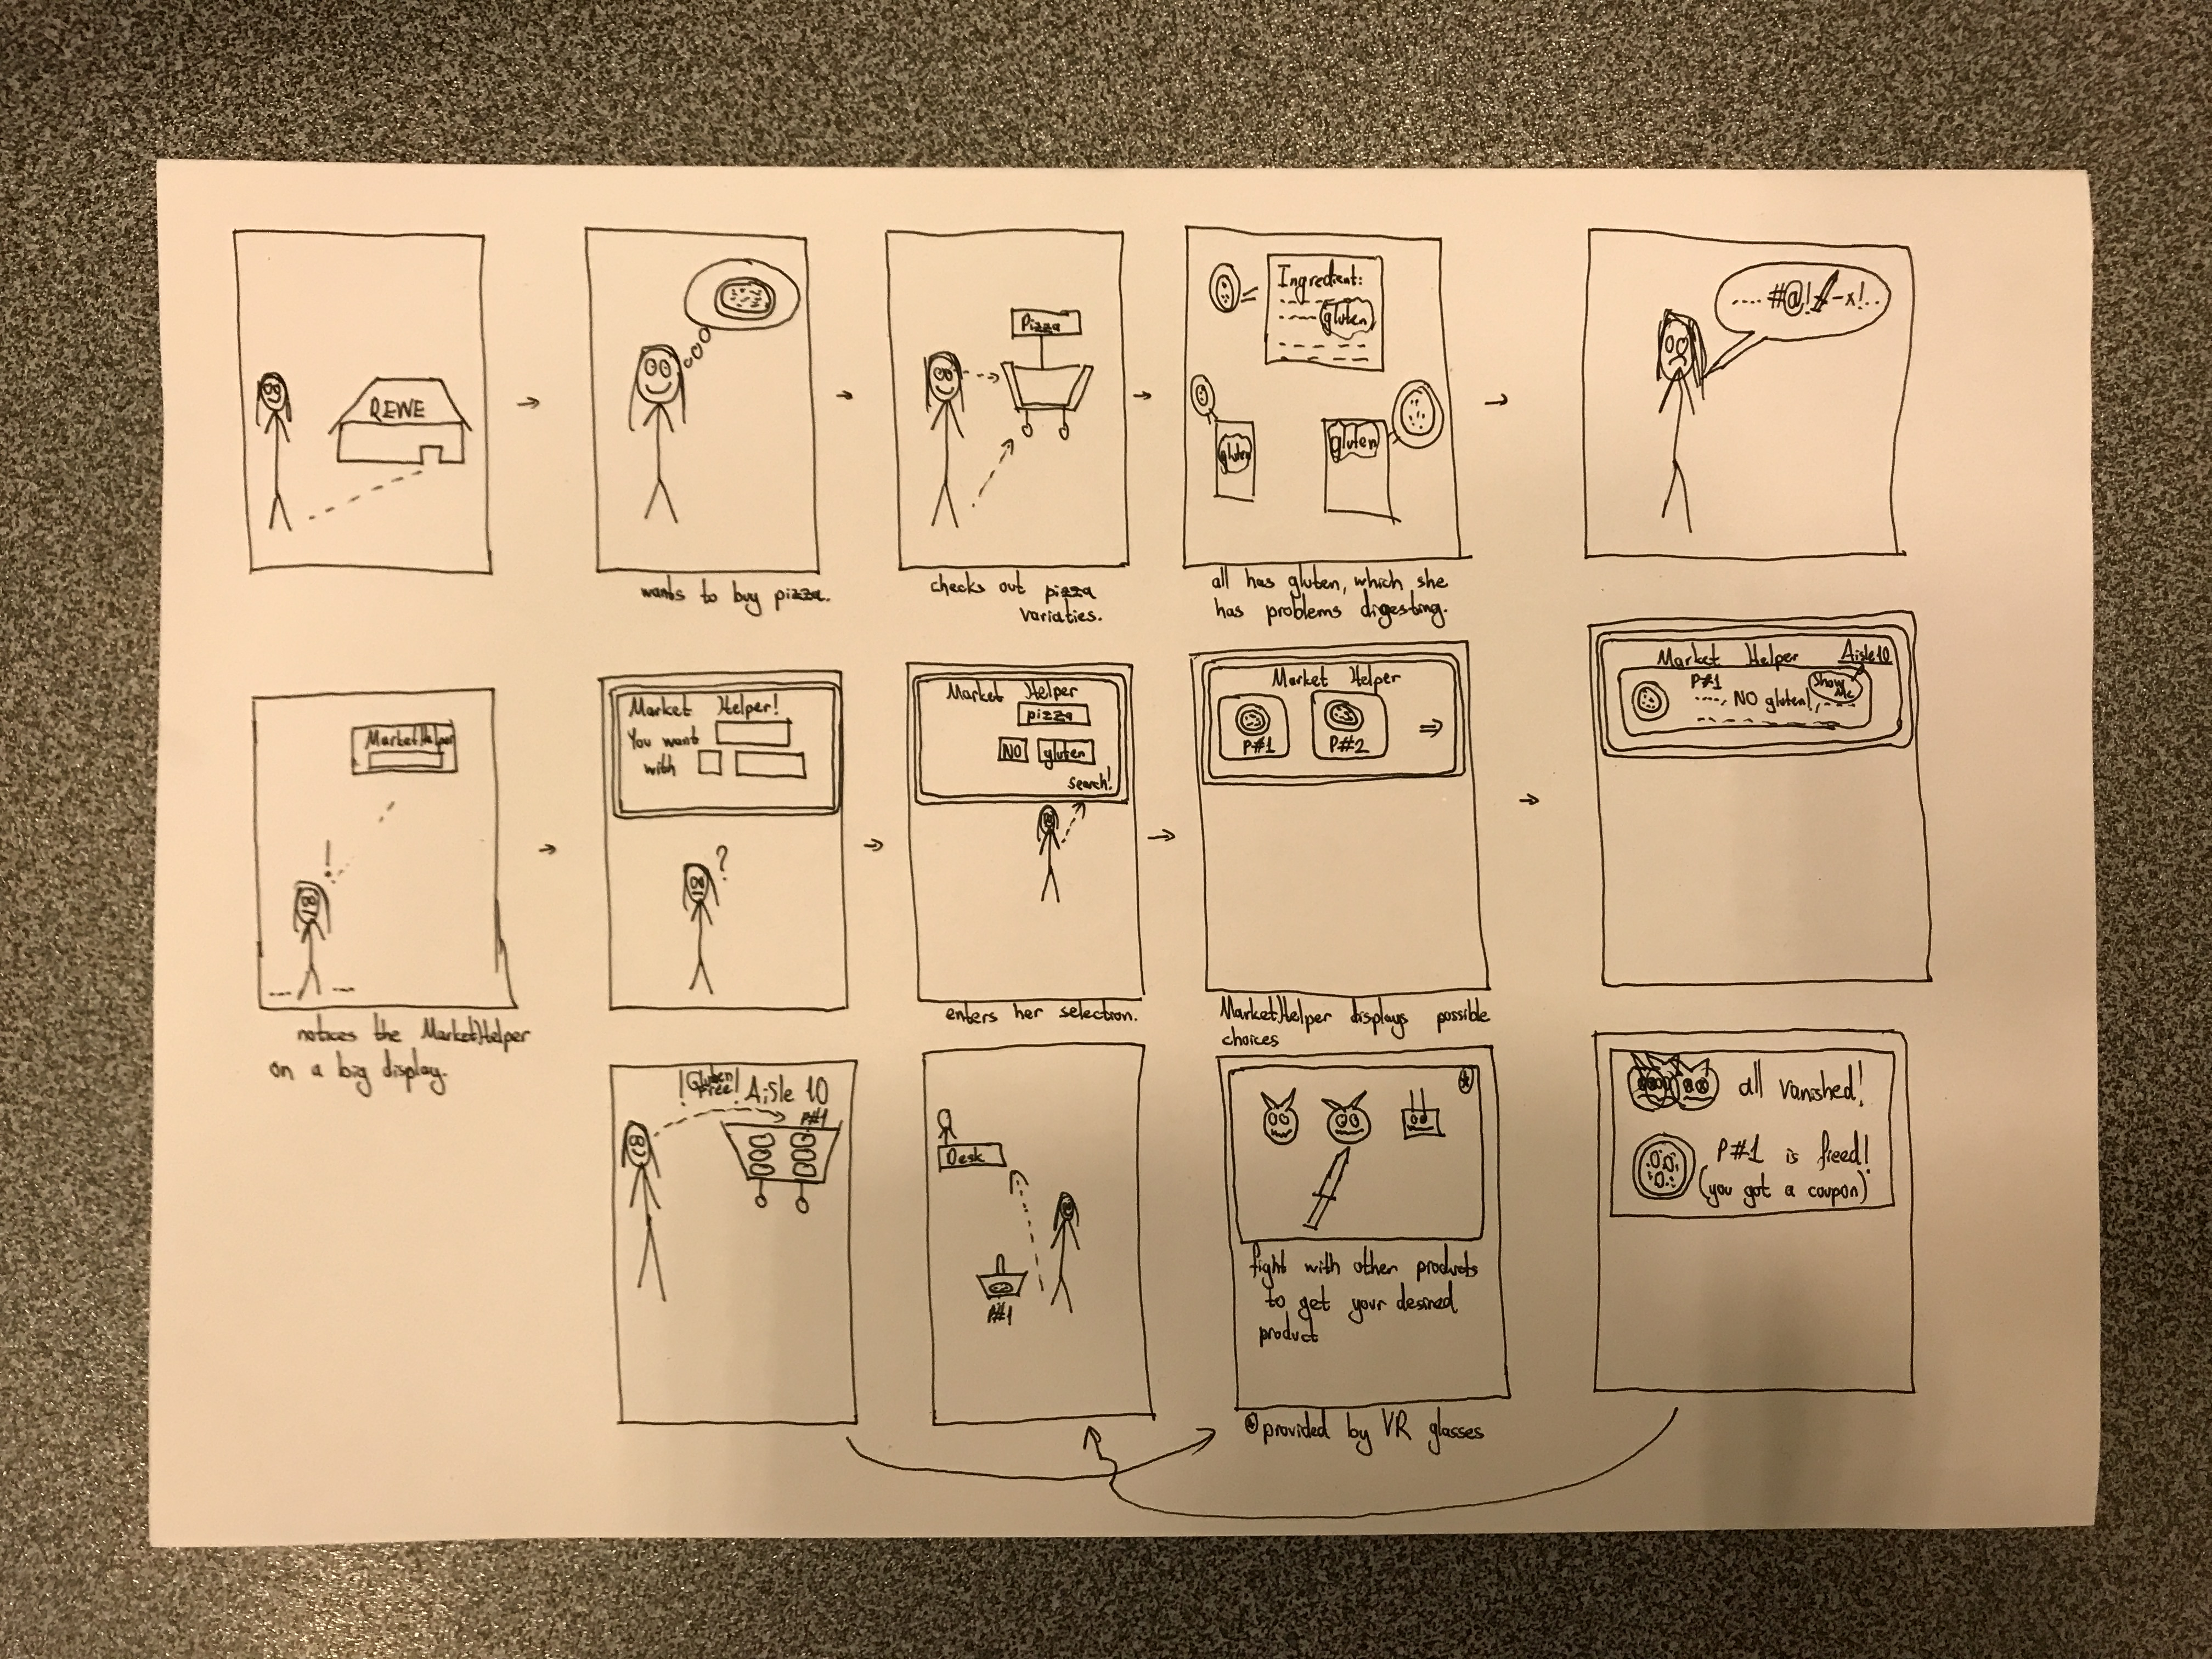
\includegraphics[scale=0.16, clip, trim={45em 0em 45em 0em}]{images/s1.jpg}
			\end{figure}
			
		\clearpage
		\subsection{Solution \#2}
		
			\noindent \textbf{Definition:}\\
			shopping assistants for supermarkets, which is placed on the handle of a shopping cart in the form of a smart tablet\\
			
			\noindent \textbf{Use Case:}\\
			Fulfilling a complete shopping list takes time, especially if users are not so aware of the layout a specific supermarket and whereabouts of the products that are needed. Asking to the employees not always help, as they are not always around or they just verbally inform once.\\
			
			Shopping List Helper! comes into play here. One can create a shopping list on the said tablet on the spot, or one can synchronize their shopping list at their phone via NFC. Then, SLH would lead the user via the shortest path either using a map of the supermarket together with the marker for the user, or via audial cues that are continuously feeded to the headphones of the user.\\
			
			\noindent \textbf{Storyboard:}\\
			
			\begin{figure}[h]
				\centering
				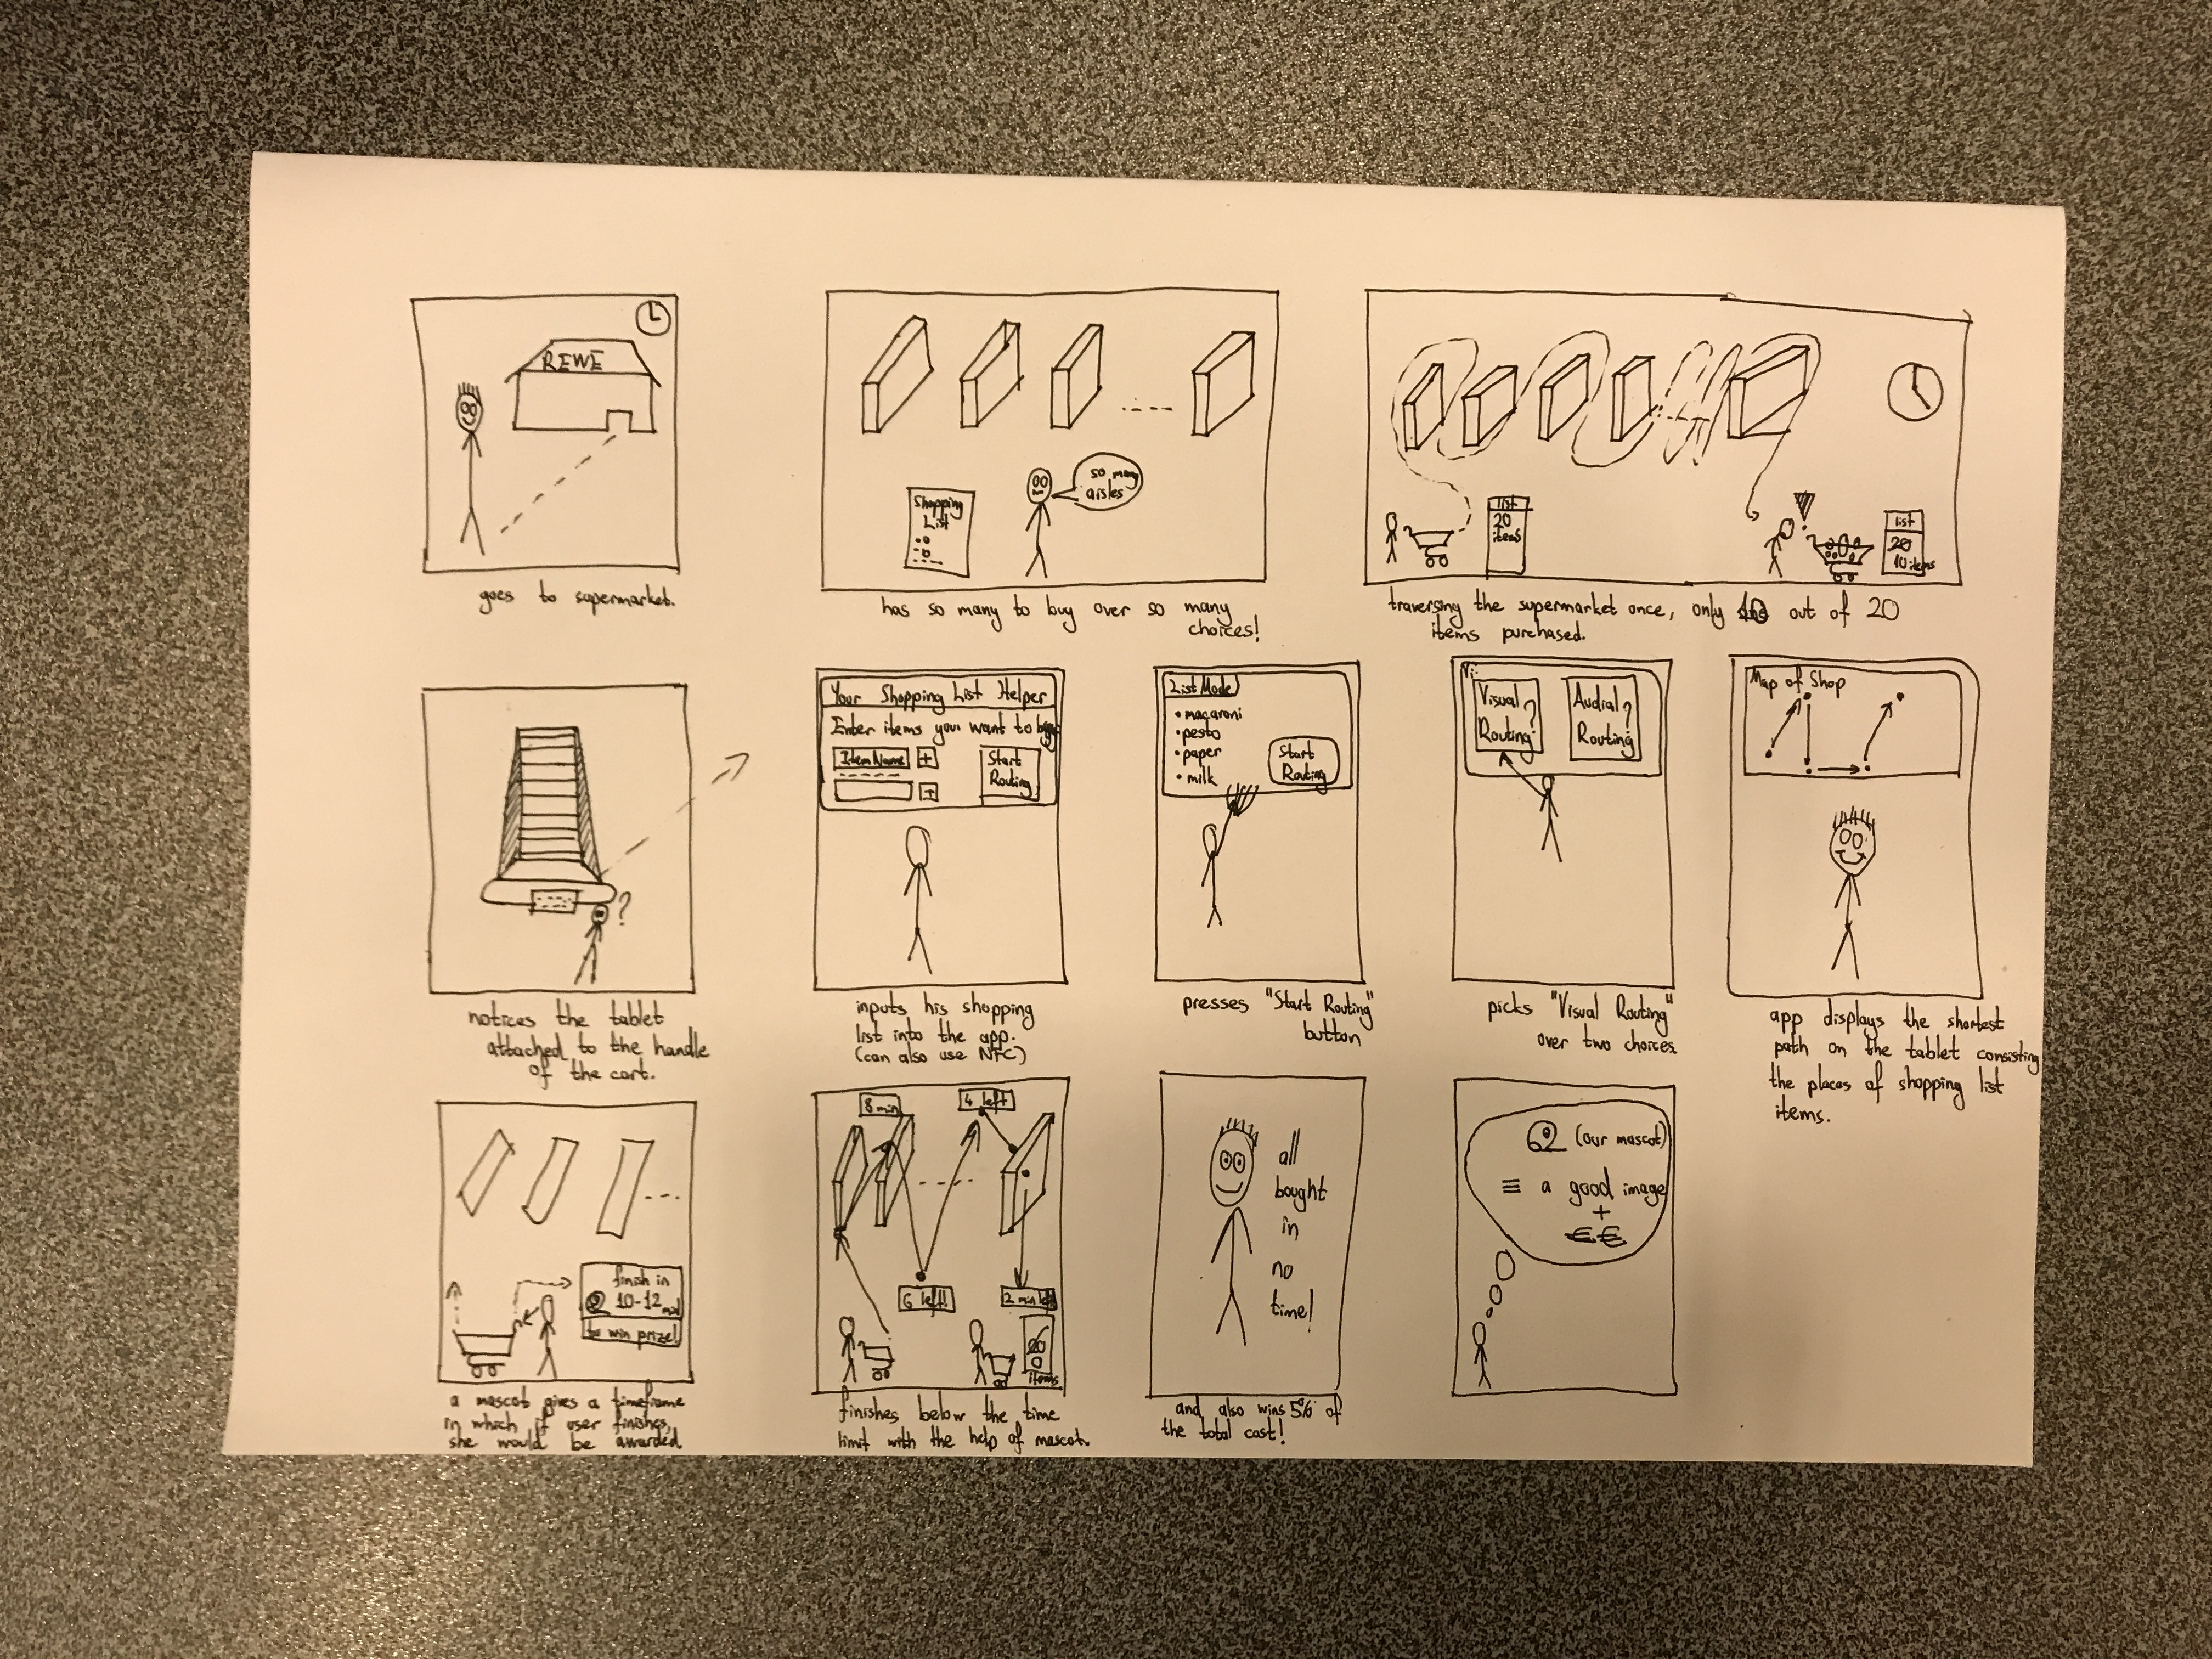
\includegraphics[scale=0.16, clip, trim={30em 0em 65em 10em}]{images/s2.jpg}
			\end{figure}
		
		\clearpage
		
		\subsection{Solution \#3}
		
		\noindent \textbf{Definition:}\\
			Meals presentation in supermarkets - user can try dish and after deciding on specific meal can take a bag with all ingredients needed to prepare the dish and go straight to the cash.\\
			
			\noindent \textbf{Use Case:}\\
			The persona "Mother" always would like to preper healthy food for her kids. She can't imagine buying fast food or already prepared dishes (put to microwave for 3 min). Once she enter to the supermarket, with our solution she will be able to get inspiration what to cook, she can try different dishes. After decision what to cook, she doesn't have to even look for ingredients, she can just take bag with all needs for specific meal.\\
		
			\noindent \textbf{Storyboard:}\\
			
			\begin{figure}[H]
				\centering
				\includegraphics[width=11cm]{example-image}
			\end{figure}
		
		\subsection{Solution \#4}
		
		\noindent \textbf{Definition:}\\
			Tablet display on refrigerator, that simply shows what ingredients do you have in the kitchen. Like self-service checkout
in the market. You can simply increase number ingredient or decrease. Then once you are in supermarket, you can get notification what ingredians you have in the kitchen.\\
			
			\noindent \textbf{Use Case:}\\
			\\
		
			\noindent \textbf{Storyboard:}\\
			
			\begin{figure}[H]
				\centering
				\includegraphics[width=11cm]{example-image}
			\end{figure}
		
		\subsection{Solution \#5}
		
			\noindent \textbf{Storyboard:}\\
			
			\begin{figure}[H]
				\centering
				\includegraphics[width=11cm]{example-image}
			\end{figure}
		
		\subsection{Solution \#6}
		
			\noindent \textbf{Storyboard:}\\
			
			\begin{figure}[H]
				\centering
				\includegraphics[width=11cm]{example-image}
			\end{figure}
		
		\bigskip
		
	\section{Six Storyboards}
		does not have to be in this order
		
	\section{Concept Map, Brainstorming Notes, Votes}
		have to include all the solutions
		
			\noindent \textbf{Concept Map:}\\
			
			\begin{figure}[H]
				\centering
				\includegraphics[width=11cm]{example-image}
			\end{figure}
		
	
	\section{Personas}
	
		\subsection{Persona \#1: Picky Eater Helga}
		
		Our extreme persona
		
		\begin{mdframed}
			\begin{minipage}{\textwidth}
				\begin{wrapfigure}{r}{0.2\textwidth}
					\centering
					\fbox{
\includegraphics[clip, trim=2cm 1cm 3cm 0cm, scale=0.63]{images/picky.jpg}}
					\vspace{-4cm}
				\end{wrapfigure}
				
				
				\textbf{Background:}\\
				25, female\\
				doing her M.Sc. in Gender Studies\\
				novice user of technology\\
				has a condition which prohibits her from eating certain foods\\
				
				
				\textbf{Motivation:}\\
				spending less time cooking food
				eating healthy
				not wasting food\\
				
				
				\textbf{Frustrations:}
				always eating the same things over and over
				making foods go to waste
				taking so much time thinking what groceries to buy
				limited options for her health condition	\\
				
				
				Meet \textbf{Helga Ratt}!\\
				
				Entertains herself reading articles on healthy food and what food has which effect on the body and the mood of a person.\\
				
				
				
				Oftenly, her health condition prevents her from eating out, and she has to look at the packaging of novel products in order to check whether they are safe for her to eat.\\
				
				
				
				Although her friends call her `health nut` once in a while, she has a good physique and healthy body, and in addition to careful meal planning, she works out to keep herself top of her game.\\
				
				She dreads spending so much time on shopping for food, as she sees shoppings as adventures first to discover new products that she can consume, then always come home with the same old tofu and like.\\
			\end{minipage}
		\end{mdframed}
	
		\subsection{Persona \#2: Mother}
		
		\textbf{Demographics:}\\
				Sarah Johnson\\
				female\\
				age: 40\\
				graduated university in Germany\\
				married\\
				mother of three kids\\
				work from 9am to 5pm\\
				living with husband and kids in rented house\\
				annual household income: 50 000 euro\\
				
		\textbf{Background:}\\
				Sarah was born and grown in Germany. She was living with parents in small countryside in the middle Germany. She he moved out from parents house when she was 18. Then Sarah moved to Frankfurt, where she started studing. She met there her current husband. After graduation, while looking for the jobs they moved to Aachen.\\
				
		\textbf{Behavior:}\\
				Sarah is very busy housewife and mother\\
				she love spend time with her husband and kids at home\\
				once a year she's going for holidays with her family\\
				she always forget things to do after, 8 hours of work. She doesn't like buying grocery products\\
				
		\textbf{Frustrations:}\\
				She is frustrated when she has to stay after hours at work. Sarah prefer to have less stressful work, even when earning less\\
				
		\textbf{Goals:}\\
				Sarah would like to spent as much time with her kids and husband at home\\
				
		
		\subsection{Persona \#3: ???}

\end{document}}
